%Victor Chavarrias (victor.chavarrias@deltares.nl)
%
%$Revision$
%$Date$
%$Author$
%$Id$
%$HeadURL$
%
%\documentclass{deltares_manual}
\documentclass{deltares_report_elv}
\svnid{$Id$}
\renewcommand{\FrontCover}{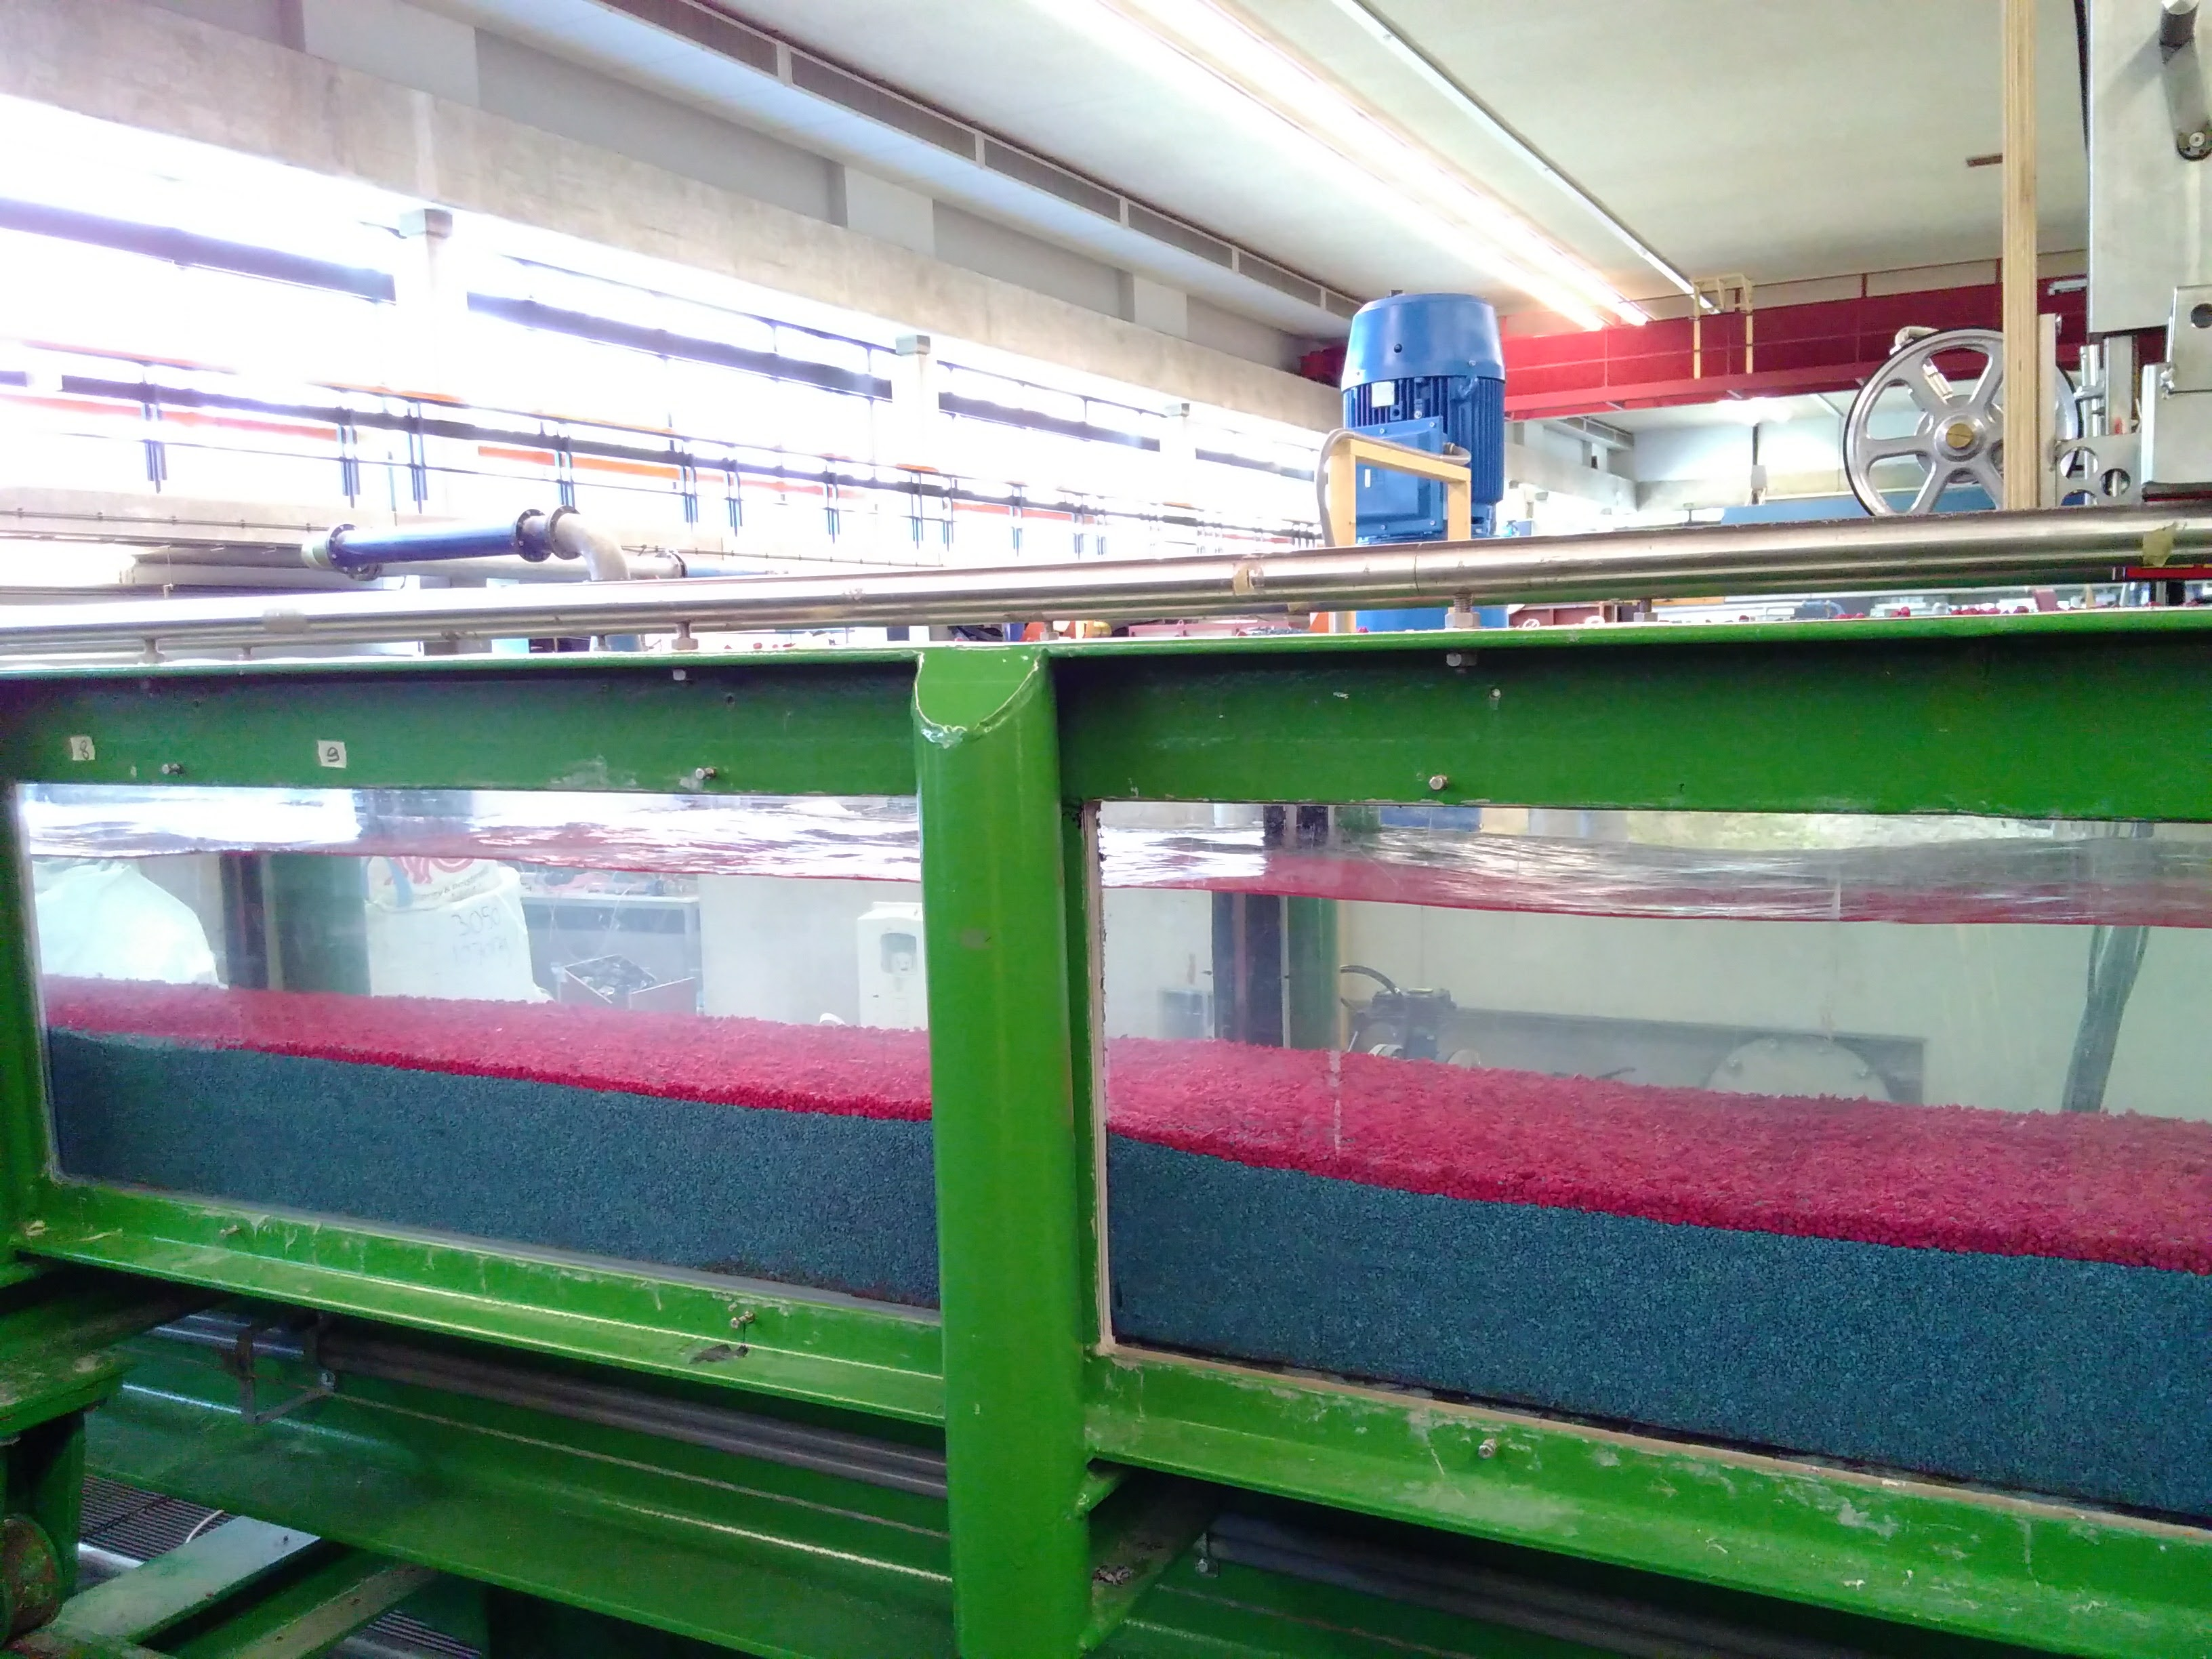
\includegraphics[height=182mm,width=182mm]{figures/cover.jpg}}

%---------references
\usepackage{natbib} %references
	\DeclareRobustCommand{\van}[3]{#2} %add \DeclareRobustCommand{\van}[3]{#3} before the bibliography

%---------math
\usepackage{array} %math arrays
\usepackage{amsmath} %math matrices
\usepackage{amssymb}
\usepackage{cancel} %cancel term in equation
\usepackage{bbm} %bold math 0 
\usepackage{bbold} %bold math characters
\usepackage{multirow} %necessary for bracket in matrix
\usepackage{bigdelim} %necessary for bracket in matrix
\usepackage{arydshln} %\hdashline[2pt/2pt] {c;{2pt/2pt}c;{2pt/2pt}c;{2pt/2pt}c}
\usepackage{upgreek} %\uppi to make \pi number and not variable

\usepackage{booktabs}

%---------include pdf
\usepackage{pdfpages} %
\usepackage{pdflscape} %\begin{landscape} \end{landscape}
%landscape
%
%\begin{landscape} 
%\includepdf[pages=-,offset=2.54cm -2.54cm,angle=0]{include/timeline.pdf}
%\end{landscape}
%portrait
%
%\includepdf[pages=-,offset=2.54cm -2.54cm]{include/CV_Erik_Mosselman.pdf}


\usepackage{graphics}
\usepackage{graphicx}
\usepackage[section]{placeins}
\graphicspath{{figures/}}
\usepackage{chngpage}

\usepackage{longtable}
%\begin{longtable}{rrp{3cm}}
%			\hline		
%			river km & date & water discharge at Lobith [\si{m^3/s}]	 \\
%			\midrule
%			\endhead
%\input{figures/adcp/measurements_overview/measurements_overview.tex} \\ %for some misterious reason, when updating the packages I needed to add this for \bottomrule not have a
%			\bottomrule
%		\caption{Summary of all ADCP profiles along the Waal River.}
%		\label{tab:table_prepos_all_all}
%\end{longtable}


%---------currency 
%use as:
%\EURO{EUR}{49500.54}
\usepackage{eurosym} 
\usepackage{euro}
\EUROSYM{EUR}{\euro}
\EUROFORMAT{main}{\out} 
\EUROFORMAT{all}{%
\form{\,}{.}{\,}%
\round{-2}%
\zero{0}{0}{}%
\plus{}{}%
\minus{\(-\)}{}
}
%
%align in table:
%\newcommand*\ALNUM{%
%\EUROFORMAT{main}{\table\out}%
%\EUROFORMAT{out}{\align\val}% % no symbol/ISO code
%\EURO{EUR}}%
%
%\begin{table}[ht]
%	\begin{center}
%	%\begin{adjustwidth}{-2cm}{-2cm}
%		\begin{tabular}{lr}		
%			\toprule
%			Fase & Coste [\euro] \\
%			\midrule
%\phaseA & \ALNUM{7000}\\
%\phaseB & \ALNUM{15000}\\
%			\bottomrule
%		\end{tabular}
%		\caption{Desglose de costes.}
%		\label{tab:costes}
%		%\end{adjustwidth}
%	\end{center}
%\end{table}
%
%different currency
%use as:
%\COP{49500.54}
%\newcommand*\COP[1]{
%{%
%\EUROFORMAT{main}{\in}%
%\EUROFORMAT{in}{\val\,COP}%
%\EUROFORMAT{EUR}{\form{\,}{.}{.}
%\round{-2}}%
%\EURO{EUR}{#1}}
%}

\usepackage{svn}
\usepackage{enumitem}

\usepackage{siunitx} %SI units

\usepackage{alphalph} %after \appendix add \renewcommand\thesection{\AlphAlph{\value{section}}} 

%figure number reset after chapter
%\usepackage{chngcntr}
%\counterwithin{figure}{chapter}

\newcommand{\addAppendix}{0} %0=no appendix; 1=add appendix
%\ifnum \addAppendix=1
%
%\fi % End of addAppendix

%general
\newcommand{\RWS}{\textit{Rijkswaterstaat~}}
\newcommand{\matlab}{Matlab\textregistered~}
\newcommand{\errmessagedisp}[1]{\errmessage{#1}\textcolor{red}{#1}}

%d3d
\newcommand{\morfac}{\textsc{MorFac}~}
\newcommand{\dtd}{Delft3D-Flow~}
\newcommand{\fm}{Delft3D-FM~}
\newcommand{\fmod}{Delft3D-FM 1D~}
\newcommand{\st}{\textsc{Sobek-3}~}
\newcommand{\waqua}{\textsc{WAQUA}~}
\newcommand{\dhydro}{D-HYDRO Suite~}
\newcommand{\sre}{\textsc{Sobek-RE}~}
\newcommand{\srur}{\textsc{Sobek-RUR}~}
\newcommand{\waqprof}{\textsc{WAQ2Prof}~}
\newcommand{\baseline}{\textsc{Baseline}~}
\newcommand{\ELV}{\textsc{ELV}}

%branches
\newcommand{\rbr}{Rhein - Boven-Rijn~}
\newcommand{\wa}{Waal~}
\newcommand{\pk}{Pannerdensh Kanaal~}
\newcommand{\nrl}{Nederrijn - Lek~}
\newcommand{\ijs}{IJssel~}
	
%math
\newcommand{\La}{L_{\mathrm{a}}}
\newcommand{\mathsub}[2]{#1_{\mathrm{#2}}}
\newcommand{\Fr}{\mathrm{Fr}}

\begin{document}
\title{\ELV}
\subtitle{Technical reference manual}
\version{\svnrev}

\author{Victor Chavarrias
}
\partner{}
\coverPhoto{Frontpage: Laboratory experiment at the TU Delft modelled using \ELV.}
\date{\today}
\references{}


%authors
\authorboxi{Victor Chavarrias}
\organisationi{Deltares}

\authori{Victor Chavarrias}

\client{}
\contact{}
\keywords{}
\reference{}
\classification{}
\status{technical reference manual}
\disclaimer{}
\projectnumber{}
\documentid{}
\summary{}
%\memoTo{ELV users}
%\memoConfidentialUntil{}
%\memoDate{\today~\currenttime}
%\memoVersion{-}
%\memoFrom{
%Victor Chavarrias 
%\;\;\;\;\;\;\;\;\;\;\;\;\;\;\;\;\;\;\;\;\;\;\;\;\;\;\;\;\;\;\;\;\;\;\;\;\;\
 %Willem Ottevanger
 %}
%\memoTelephone{
%+31\,(0)88\,335\,8033 
%\;\;\;\;\;\;\;\;\;\;\;\;\;\;\;\;\;\;\;\;\;\;\;\;\;\;\;\;\;\;\;\;\;\;\;\;\;\
%+31\,(0)88\,335\,8532
%}
%\memoEmail{
%victor.chavarrias@deltares.nl 
%willem.ottevanger@deltares.nl
%}
%\memoSubject{Implementation of the Preissmann scheme in \ELV}
%\memoCopy{-}

\deltarestitle

\newpage

\chapter{Introduction}

\ELV{} is a open-source software written in Matlab for modelling one-dimensional river morphodynamic processes ideal for research purposes.

Victor Chavarrias started it on the 23$^{\text{rd}}$ of February of 2016. Liselot Arkesteijn has implemented several features as well inestimable support and ideas. Pepijn van Denderen implemented the possibility of modelling several branches. The first backwater solver is thanks to Guglielmo Stecca. 

\chapter{Code structure}

\newcommand{\codeInit}{Initialization}
\newcommand{\codeTimeLoop}{Time loop}
	\newcommand{\codeFlowUpdate}{Flow update}
	\newcommand{\codeFriction}{Friction correction}
	\newcommand{\codeSedTrans}{Sediment transport}
	\newcommand{\codeInterpolate}{Interpolation}
	\newcommand{\codeStruiksma}{Struiksma reduction}
	\newcommand{\codeParticleActivity}{Particle activity}
	\newcommand{\codeNodalPoint}{Nodal point relation}
	\newcommand{\codeBedLevelUpdate}{Bed level update}
	\newcommand{\codeLaUpdate}{Active layer thickness update}
	\newcommand{\codeGSDUpdate}{Grain size distribution update}
	\newcommand{\codeFrictionUpdate}{Friction update}
	\newcommand{\codeResultsWriting}{Results writing}
	\newcommand{\codeTimeStep}{Time step computation}
\newcommand{\codeFinal}{Finalization}

The code structure is:
\begin{enumerate}[label*=\arabic*.]
\item \codeInit{} (Section \ref{sec:codeInit})
%\item \codeTimeLoop (Section \ref{sec:codeTimeLoop}})
\item \codeTimeLoop{} 
\begin{enumerate}[label*=\arabic*.]
\item \codeFlowUpdate{} (Section \ref{sec:codeFlowUpdate})
\item \codeFriction{} (Section \ref{sec:codeFriction})
\item \codeSedTrans{} (Section \ref{sec:codeSedTrans})
\item \codeInterpolate{} (Section \ref{sec:codeInterpolate})
\item \codeStruiksma{} (Section \ref{sec:codeStruiksma})
\item \codeParticleActivity{} (Section \ref{sec:codeParticleActivity})
\item \codeNodalPoint{} (Section \ref{sec:codeNodalPoint})
\item \codeBedLevelUpdate{} (Section \ref{sec:codeBedLevelUpdate})
\item \codeLaUpdate{} (Section \ref{sec:codeLaUpdate})
\item \codeGSDUpdate{} (Section \ref{sec:codeGSDUpdate})
\item \codeFrictionUpdate{} (Section \ref{sec:codeFrictionUpdate})
\item \codeResultsWriting{} (Section \ref{sec:codeResultsWriting})
\item \codeTimeStep{} (Section \ref{sec:codeTimeStep})
\end{enumerate}
\item{\codeFinal{}}
\end{enumerate}

\section{\codeInit{}}
\label{sec:codeInit}

The space domain $x$ is discretized into $M$ cells of equal length $\Delta x$ [\si{m}]. The equations are solved in a one-dimensional domain of length $L$ [\si{m}] extending from $x=\mathsub{x}{o}$ until $x=\mathsub{x}{f}$ over time $T$ [\si{s}] between $t=\mathsub{t}{1}$ and $t=\mathsub{t}{2}$. 

\section{\codeFlowUpdate{}}
\label{sec:codeFlowUpdate}

\subsection{Physical system of equations}

%\subsection{Set of equations}

The \citet{SaintVenant71} equations in conservative form read:
\begin{equation}
\label{eq:sv_mass}
\frac{\partial h}{\partial t}+\frac{\partial q}{\partial x}=0 \;,
\end{equation}
\begin{equation}
\label{eq:sv_mom}
\frac{\partial q}{\partial t}+\frac{\partial q^2/h}{\partial x}+\frac{1}{2}g\frac{\partial h^2}{\partial x}+gh\frac{\partial \eta}{\partial x}=-C_f\frac{q^2}{h^2} \;.
\end{equation}

In solving the flow equations, $g$ and $\mathsub{C}{f}$ are assumed constant and $\eta$ constant in time.


%\subsection{Linearization of the system of equations}
%
%We consider a reference state that is a solution to the system of equations. The reference state is a steady uniform straight flow in the $x$ direction over an inclined plane bed. Mathematically: $h_0=\text{ct.}$, $q_0=\text{ct.}$, $\frac{\partial \eta}{\partial x}=\text{ct.}=\frac{-\mathsub{C}{f}{q_0}^2}{gh_0^3}$, where ct.\ denotes a constant different from 0 and subscript $0$ indicates the reference solution. 
%
%We add a small perturbation to the reference solution denoted by $'$ and we linearise the resulting system of equations. After substituting the reference solution we obtain a system of equations of the perturbed variables:
%\begin{equation}
%\label{eq:matrixf_sf}
	%\frac{\partial \mathbf{G'}}{\partial t}+\mathbf{C_{0}}\frac{\partial \mathbf{G'}}{\partial x}+\mathbf{B_0}\mathbf{G'}=0 \;,
%\end{equation}
%where the vector of dependent variables is:
%\begin{equation}
%\label{eq:Q_l}
	%\mathbf{G'}=\left[h',q'\right]^{\intercal} \;,
%\end{equation}
%
%The advective matrix in $x$ direction is:
%\begin{equation}
%\label{eq:Ax_sf}
%\makebox[\textwidth][c]{$
		%\mathbf{C_{0}}=\left[
 %\begin{array}{cc}
%%wmass 
  %0 & 1  \\
%%water mom x
	%gh_0-\left(\frac{q_{\mathrm{x}0}}{h_0}\right)^2 & 2\frac{q_{\mathrm{x}0}}{h_0} \\
 %\end{array}\right] \;.
%$}
%\end{equation}
%
%The matrix of linear terms is:
%\begin{equation}
%\label{eq:B}
%\makebox[\textwidth][c]{$
		%\mathbf{B_0}=\left[
		%\begin{array}{cc}
  %0 & 0 \\
	%\frac{-3C_{\mathrm{f}}q_{\mathrm{x}0}^2}{h_0^3} & \frac{2C_{\mathrm{f}}q_{\mathrm{x}0}}{h_0^2} \\
 %\end{array}\right] \;.
%$}
%\end{equation}

%\subsection{Boundary conditions}



At $t=\mathsub{t}{1}$, $h=\mathsub{H}{1}(x)$ and $q=\mathsub{Q}{1}(x)$ for $\mathsub{x}{o}\leq x \leq\mathsub{x}{f}$.

At $x=\mathsub{x}{o}$, $q=\mathsub{Q}{o}(x)$ for $\mathsub{t}{1}\leq t \leq\mathsub{t}{2}$.

At $x=\mathsub{x}{f}$, $h=\mathsub{H}{f}(x)$ for $\mathsub{t}{1}\leq t \leq\mathsub{t}{2}$.

\subsection{Numerical discretization}

The non-linear set of equations (\ref{eq:sv_mass})-(\ref{eq:sv_mom}) is discretized at the cell centres by means of the $\theta$-box scheme:
\begin{equation}
\frac{\partial f}{\partial t}=\frac{1}{2}\left(\frac{f_{m+1}^{n+1}-f_{m+1}^{n}}{\Delta t}+\frac{f_{m}^{n+1}-f_{m}^{n}}{\Delta t}\right) \;,
\end{equation}
\begin{equation}
\frac{\partial f}{\partial x}=\theta\left(\frac{f_{m+1}^{n+1}-f_{m}^{n+1}}{\Delta x}\right)+\left(1-\theta\right)\left(\frac{f_{m+1}^{n}-f_{m}^{n}}{\Delta x}\right) \;,
\end{equation}
where $\theta\in[0.5,1]$ is a parameter, $m\in[1,N]$ is an index indicating cell centre number in increasing order, and $n>1$ is an index indicating time. 

For $\theta=0.5$ one obtains the Preissmann scheme \citep{Preissmann61_2,Preissmann61_3,Lyn87_2}.


The first term in Equation (\ref{eq:sv_mass}) is:
%\begin{equation}

%\end{equation}

The slope is approximated as:
\begin{equation}
\left.\frac{\partial \eta}{\partial x}\right|_{m}=\frac{\eta_{m+1}-\eta_{m}}{\Delta x} \;,
\end{equation}



%\errmessage{Jacobian terms}

\subsection{Solution of the algebraic system of equations}

The discretized set of equations form a system of algebraic equations:
\begin{equation}
\label{eq:alg}
\mathbf{A}\left(\mathbf{Q}^{n+1}\right)\mathbf{Q}^{n+1}=\mathbf{B}\left(\mathbf{Q}^{n}\right)\;.
\end{equation}

Vector:
\begin{equation}
\mathbf{Q}^{n+1}=[h_1^{n+1}, h_2^{n+1}, \cdots, h_{M-1}^{n+1}, h_M^{n+1}, q_1^{n+1}, q_2^{n+1}, \cdots, q_{M-1}^{n+1}, q_M^{n+1}]^{\intercal} \;,
\end{equation}
is the $2N$x1 vector of unknowns. 

Matrix:
\begin{equation}
\makebox[\textwidth][c]{$
		\mathbf{A}\left(\mathbf{Q}^{n+1}\right)=\left[
		\begin{array}{cc}
  \mathbf{A}_{1}(\mathbf{Q}^{n+1}\right) & \mathbf{A}_{2}(\mathbf{Q}^{n+1}\right) \\
	\mathbf{A}_{3}(\mathbf{Q}^{n+1}\right) & \mathbf{A}_{4}(\mathbf{Q}^{n+1}\right) \\
 \end{array}\right] \;,
$} 
\end{equation}
is the $2N$x$2N$ matrix containing the implicit terms, which is subdivided into 4 $N$x$N$ submatrices.

Vector:
\begin{equation}
\makebox[\textwidth][c]{$
		\mathbf{B}\left(\mathbf{Q}^{n}\right)^{n}=\left[
		\begin{array}{cc}
  \mathbf{B}_{1}\left(\mathbf{Q}^{n}\right)\\
	\mathbf{B}_{2}\left(\mathbf{Q}^{n}\right)\\
 \end{array}\right] \;,
$} 
\end{equation}
is the $2N$x1 vector of explicit terms. 

The system is solved using the Newton–Raphson method until $r<\epsilon$:
\begin{equation}
\label{eq:nr}
\mathbf{Q}^{j+1}=\mathbf{Q}^{j}-(\mathbf{J_0}^{j})^{-1}\left(\mathbf{A}^{j}\mathbf{Q}^{j}-\mathbf{B}^{j}\right) \;,
\end{equation}
where $j$ is the iteration index. The operation to the right of equation (\ref{eq:nr}) is done using function \texttt{mldivide} applied to arguments $\mathbf{J_0}^{j}$ and $\mathbf{A}^{j}\mathbf{Q}^{j}-\mathbf{B}^{j}$. The residual $r$ is computed as:
\begin{equation}
r=\max{\left|\left(\mathbf{A}^{j}\mathbf{Q}^{j}-\mathbf{B}^{j}\right)\right|} \;.
\end{equation}

\section{\codeFriction{}}
\label{sec:codeFriction}

\section{\codeSedTrans{}}
\label{sec:codeSedTrans}

\section{\codeInterpolate{}}
\label{sec:codeInterpolate}

Some functions require information at cell edges ($m-1/2$ and $m+1/2$). This is done by linear interpolation. Extrapolation is applied at the first and last cells.

\section{\codeStruiksma{}}
\label{sec:codeStruiksma}

\section{\codeParticleActivity{}}
\label{sec:codeParticleActivity}

\section{\codeNodalPoint{}}
\label{sec:codeNodalPoint}

\section{\codeBedLevelUpdate{}}
\label{sec:codeBedLevelUpdate}

\subsection{Physical system of equations}

Mass conservation of sediment is solved in its flux form (Section \ref{sec:exner_flux}):
\begin{equation}
\label{eq:exner_flux}
\frac{\partial \eta}{\partial t}+\frac{\mathsub{M}{f}}{\mathsub{c}{b}\beta}\frac{\partial \mathsub{q}{b}}{\partial x}=0 \;,
\end{equation}
or in entrainment-deposition form (Section \ref{sec:exner_ed}):
\begin{equation}
\frac{\partial \eta}{\partial t}=\frac{\mathsub{M}{f}}{\mathsub{c}{b}}\left(D-E\right)=0 \;.
\end{equation}

\subsection{Numerical discretization of the flux form}
\label{sec:exner_ed}

\newcommand{\BorsboomScheme}{Borsboom scheme}

The flux version (Equation \ref{eq:exner_flux}) can be solved using a FTBS (Forward in Time and Backward in Space) scheme (Section \ref{sec:exner_ftbs}) or the \BorsboomScheme{} (Section \ref{sec:BorsboomScheme}). 

\subsubsection{FTBS}
\label{sec:exner_FTBS}

\begin{equation}
\eta_{m}^{n+1}=\eta_{m}^{n}-\frac{\mathsub{M}{f}\Delta t}{\mathsub{c}{b}\beta_{m}\Delta x}\left(\left.\mathsub{q}{b}\right._{m-1}^{n}-\left.\mathsub{q}{b}\right._{m}^{n}\right)
\end{equation}

\subsubsection{\BorsboomScheme{}}

The bed elevation at the cell centre of the first and last two cells is found applying FTBS (Section \ref{sec:exner_FTBS}). 

The remaining cell centre bed elevation is updated as:
\begin{equation}
\label{eq:exner_borsboom}
\eta_{m}^{n+1}=\eta_{m}^{n}-\frac{\mathsub{M}{f}\Delta t}{\mathsub{c}{b}\beta_{m}\Delta x}\left(\varphi_{m-1/2}^{n}-\varphi_{m+1/2}^{n}\right) \;,
\end{equation}
%
\begin{equation}
\label{eq:phi_borsboom}
\varphi_{m-1/2}=\left.\mathsub{q}{b}\right._{m-1/2}+\frac{1}{2}c_{m-1/2}\left[\left(1-\left.\mathsub{\sigma}{b}\right._{m-1/2}\right)\Phi_{m-1}-1\right]\left(\eta_{m}-\eta_{m-1}\right) \;,
\end{equation}
%
\begin{equation}
\label{eq:sigma_borsboom}
\left.\mathsub{\sigma}{b}\right._{m-1/2}=c_{m-1/2}\frac{\Delta t}{\Delta x} \;,
\end{equation}
%
\begin{equation}
\label{eq:sigma_borsboom}
\left.\mathsub{\sigma}{b}\right._{m-1/2}=c_{m-1/2}\frac{\Delta t}{\Delta x} \;,
\end{equation}
%
$\phi_{m}$ is a flux limiter (Appendix \ref{app:flux_lim}) based on $r_{m}$:
\begin{equation}
\label{eq:r_borsboom}
r_{m}=\frac{\eta_m-\eta_{m-1}}{\eta_{m+1}-\eta_m+\epsilon} \;,
\end{equation}
where $\epsilon=\num{1e-10}$ is a tolerance. 
%
$c$ is the bed celerity (Appendix \ref{sec:celerities})

\subsection{Numerical discretization of the entrainment-deposition form}
\label{sec:exner_ed}

\section{\codeLaUpdate{}}
\label{sec:codeLaUpdate}

\section{\codeGSDUpdate{}}
\label{sec:codeGSDUpdate}

\section{\codeFrictionUpdate{}}
\label{sec:codeFrictionUpdate}

\section{\codeResultsWriting{}}
\label{sec:codeResultsWriting}

\section{\codeTimeStep{}}
\label{sec:codeTimeStep}

\section{\codeFinal{}}
\label{sec:codeFinal}

%\begin{figure}[ht]
    %\centering
    %\includegraphics[width=\textwidth]{carraro.png}
		%\caption{Propagation of a sediment hump under steady flow condition (Figure from \citet{Carraro18_2}).}
    %\label{fig:carraro}
%\end{figure}
%
%\begin{table}[ht]
	%\begin{center}
	%\begin{adjustwidth}{-2cm}{-2cm}
		%\begin{tabular}{clcrc}		
			%\toprule
			%Case & Model & Sediment fraction(s) & Mobility & $\alpha_{\mathrm{m}}$  \\
			%\midrule
%S1 & Struiksma & fine & - &  - \\ %151
%S2 & Hirano & fine \& coarse & - & - \\ %129
%S3 & Adapted coarse layer & fine \& coarse& Shields (discrete)& 1 \\ %150
%S4 & Adapted coarse layer & fine \& coarse& Shields (continuous)& 1 \\ %153 
%S5 & Adapted coarse layer & fine \& coarse& Wilcock and McArdell (continous) & 1 \\ %154
%\midrule
%S6 & Adapted coarse layer & fine \& coarse& Shields (discrete)& 20 \\ %157
%S7 & Adapted coarse layer & 2 x fine \& coarse& Shields (discrete)& 1 \\ %158
			%\bottomrule
		%\end{tabular}
		%\caption{Simulations to model the T2 flume experiment of \citet{Struiksma99}.}
		%\label{tab:ini_diff}
		%\end{adjustwidth}
	%\end{center}
%\end{table}
%
%
%
%\section{Discussion}

\newpage
\appendix
\renewcommand\thesection{\AlphAlph{\value{section}}}

\chapter{Variables}

\begin{longtable}{|p{1.5cm}|p{1.5cm}|p{10cm}|}
\caption{Variables in \ELV{}}\\
\hline
\textbf{Symbol} & \textbf{Unit} & \textbf{Meaning} \\
\hline
\endfirsthead
\multicolumn{3}{c}%
{\tablename\ \thetable\ -- \textit{Continued from previous page}} \\
\hline
%\textbf{First entry} & \textbf{Second entry} & \textbf{Third entry} & \textbf{Fourth entry} \\
\hline
\endhead
\hline \multicolumn{3}{r}{\textit{Continued on next page}} \\
\endfoot
\hline
\endlastfoot
$c$ & \si{m/s} & bed celerity \\
$c^{*}$ & \si{m/s} & non-dimensional bed celerity \\
$\mathsub{c}{b}$ & - & 1-porosity \\
$\mathsub{C}{f}$ & - & non-dimensional friction coefficient \\
$D$ & \si{m/s} & Deposition rate \\
$E$ & \si{m/s} & Entrainment rate \\
$\Fr{}$ & - & Froude number \\
$g$ & \si{m/s^2} & acceleration due to gravity \\
$h$ & \si{m} & flow depth \\
$m$ & - & index of the cell centre \\
$M$ & - & number of cells in the domain \\
$n$ & - & index of time \\
$\mathsub{M}{f}$ & - & morphodynamic acceleration factor \\
$q$ & \si{m^2/s} & discharge per unit width \\
$\mathsub{q}{b}$ & \si{m^2/s} & sediment discharge per unit width \\
$t$ & \si{s} & time coordinate \\
$x$ & \si{m} & streamwise coordinate \\
$\alpha$ & - & preconditioning variable for volume fraction content\\
$\beta$ & - & preconditioning variable for bed elevation\\
$\Delta t$ & \si{s} & time step \\
$\Delta x$ & \si{m} & space step \\
$\Phi$ & - & flux limiter \\
$\eta$ & \si{m} & bed elevation \\ 
$\mathsub{\sigma}{b}$ & - & CFL number of the bed \\
\end{longtable}

\chapter{Flux limiters}
\label{app:flux_lim}

\section{Koren}

\begin{equation}
\Phi=\max\left(0,\min\left(2,\min\left(2+\frac{r}{3},2r\right)\right)\right)
\end{equation}

\chapter{Celerities}
\label{sec:celerities}

The bed celerity is computed as:
\begin{equation}
\label{eq:c_bed}
c=\frac{\mathsub{M}{f}u}{\mathsub{c}{b}\beta}c^{*}\;,
MorFac*u.*celerities.lb./(1-porosity)./beta
\end{equation}
%
where the non-dimensional bed celerity $c*$ [-] is computed as:
\begin{equation}
\label{eq:c_bed_nondim}
c^{*}=\frac{\psi}{1-\Fr{}^2}\;,
\end{equation}
\begin{equation}
\label{eq:psi}
\psi=\frac{\partial \mathsub{q}{b}}{\partial u} \;,
\end{equation}
where the derivative is computed with finite differences. 

\end{document}

%
%
%
%----------------------------
%---------BIBLIOGRAPHY
%----------------------------
%
\newpage
\section*{References}
\DeclareRobustCommand{\van}[3]{#3}
%\bibliographystyle{agufull08_mod}
\bibliography{../references/references}

%\includepdf[pages=-]{include/timeline.pdf} 

\LastPage
\end{document}
